% Introduction
%!TEX root = ../Project.tex

\section{Introduction} 
\label{introduction}
       
An RPG (Role Playing Game) is a game where a player assumes the role of a character. An RPG is usually story driven and the character usually has a quest to complete. In the course of the game the player will go to different environments such as town and dungeons. In these environments the player will have to fight opponents in battles. Combat in RPGs is normally a simple turn based system where players and their opponents take turns to attack each other using various skills\footnote{Although there are some common variants that will be discussed later on.}. 

A Tactical RPG is a sub-genre of an RPG that focuses on the combat side of the genre. A Tactical RPG is a series of \texttt{battles}, which take place in various environments intertwined with an over-arching story.

Each \texttt{battle} is grid based (like chess) where each player has a number of units(pieces). 
\begin{figure}[htbp] \centering 
	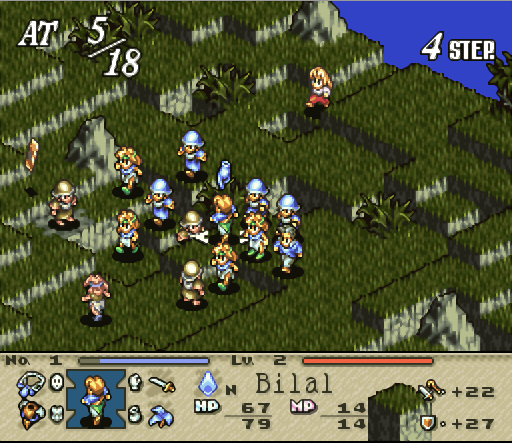
\includegraphics[height=3.5in]{figures/TRPG.png} 
	\caption{\textbf{Tactics Ogre}\cite{to} a classic Tactical RPG } 
	\label{fig:TRPG} 
\end{figure}
The players take turns to move their units. Each unit has attributes associated with it, such as strength, and hit points that affect all the actions in the game. Like chess, there are different kinds of units which have different abilities which affects how the unit moves and what actions they can perform. A unit can attack another player's units. The goal of the battle is usually to defeat all the opponent's units although other goals are possible.

The aim of this project is to create an engine which will take resources such as graphics, sounds and rules of the game to create a runnable Tactical RPG. A detailed description of the scope and goals of the project is in section \ref{sec:requirements_specification}

\subsection{Project Baseline}
\label{sub:baseline}

No previous work was used for this project. All of the project was created during the course of the academic year.

\subsection{Project Success}

Having completed all the primary and secondary objectives as well as nearly all the tertiary objectives, I would say that the project was successful.  Notable features that were accomplished include a very customisable engine which allows the user to specify most aspects of their created game and an editor which allows the user to make a complex game without \texttt{any} programming(although programming can be used to further enhance their game). 

The ability to export the user's created game as a standalone application without any external dependencies is a significant feature of the project. Since Java was used, the created game is cross-platform and can run on any system with  a complete Java runtime environment\footnote{i.e The GUI and Editor won't run on Android since it does not have the \texttt{Swing} toolkit.}.  

Results from the usability studies were very positive, with most users saying they enjoyed using the system and found it usable. 
